\documentclass[11pt]{article}
\usepackage[margin=1in]{geometry}
\usepackage{pgfplots}
\usepackage{pgfplotstable}
\usepackage{tikz}
\usepackage{filecontents}
\usepackage{subcaption}
\usepackage{amsmath}
\usepackage{multirow}
\usepackage{pdflscape}
\usepackage{booktabs}

\pgfplotsset{compat=1.17}
\usepgfplotslibrary{statistics}
\usepgfplotslibrary{fillbetween}

% Include shared styles
% Define colors for different experiments
\definecolor{exp1}{RGB}{31, 119, 180}    % blue - Cuckoo 
\definecolor{exp2}{RGB}{214, 39, 40}     % red - Iceberg
\definecolor{exp3}{RGB}{127, 127, 127}   % grey - Junction
\definecolor{exp4}{RGB}{44, 160, 44}     % green - TPHT
\definecolor{exp5}{RGB}{148, 103, 189}   % purple - TBB
\definecolor{exp6}{RGB}{255, 127, 14}     % yellow - Blast
\definecolor{poisson}{RGB}{148, 103, 189} % purple - for theoretical plots

% Define bar styles for each object (used in bar charts)
\pgfplotsset{
    CuckooBarStyle/.style={fill=exp1!35, draw=exp1!80},
    IcebergBarStyle/.style={fill=exp2!35, draw=exp2!80},
    JunctionBarStyle/.style={fill=exp3!35, draw=exp3!80},
    TPHTBarStyle/.style={fill=exp4!35, draw=exp4!80},
    TBBBarStyle/.style={fill=exp5!35, draw=exp5!80},
    BlastBarStyle/.style={fill=exp6!35, draw=exp6!80},
    % Macro-based aliases
    htthreeBarStyle/.style={CuckooBarStyle},
    htfourBarStyle/.style={IcebergBarStyle},
    htfiveBarStyle/.style={JunctionBarStyle},
    htoneBarStyle/.style={TPHTBarStyle},
    htsixBarStyle/.style={TBBBarStyle},
    httwoBarStyle/.style={BlastBarStyle}
} 

% Define line styles for each object (used in line/scatter charts)
\pgfplotsset{
    CuckooLineStyle/.style={color=exp1, mark=o, mark size=2.5pt, thick, smooth},
    IcebergLineStyle/.style={color=exp2, mark=square, mark size=2.5pt, thick, smooth},
    JunctionLineStyle/.style={color=exp3, mark=triangle, mark size=2.5pt, thick, smooth},
    TPHTLineStyle/.style={color=exp4, mark=diamond, mark size=2.5pt, thick, smooth},
    TBBLineStyle/.style={color=exp5, mark=star, mark size=2.5pt, thick, smooth},
    BlastLineStyle/.style={color=exp6, mark=pentagon, mark size=2.5pt, thick, smooth},
    % Macro-based aliases
    htthreeLineStyle/.style={CuckooLineStyle},
    htfourLineStyle/.style={IcebergLineStyle},
    htfiveLineStyle/.style={JunctionLineStyle},
    htoneLineStyle/.style={TPHTLineStyle},
    htsixLineStyle/.style={TBBLineStyle},
    httwoLineStyle/.style={BlastLineStyle}
}

% Additional utility styles
\pgfplotsset{
    PoissonLineStyle/.style={color=poisson, thick, smooth},
    PoissonFillStyle/.style={color=poisson!20, fill=poisson!20},
    OccScatterStyle/.style={only marks, mark=o, mark size=2.2pt, color=exp1, opacity=0.85}
}

% Semantic styles for probabilistic analysis plots
\pgfplotsset{
    InsertionOnlyStyle/.style={color=exp1, mark=o, mark size=2.5pt, thick, smooth},
    WithDeletionStyle/.style={color=poisson, mark=square, mark size=2.5pt, thick, smooth},
    PoissonTheoryStyle/.style={color=poisson, thick, smooth},
    ExperimentalBoxStyle/.style={fill=exp1!25, draw=exp1}
}

% Backward-compatible aliases for existing macros expecting these names (bar plots)
\pgfplotsset{
    CuckooStyle/.style={CuckooBarStyle},
    IcebergStyle/.style={IcebergBarStyle},
    JunctionStyle/.style={JunctionBarStyle},
    TPHTStyle/.style={TPHTBarStyle},
    TBBStyle/.style={TBBBarStyle},
    BlastStyle/.style={BlastBarStyle},
    % Additional macro-based aliases
    htthreeStyle/.style={CuckooBarStyle},
    htfourStyle/.style={IcebergBarStyle},
    htfiveStyle/.style={JunctionBarStyle},
    htoneStyle/.style={TPHTBarStyle},
    htsixStyle/.style={TBBBarStyle},
    httwoStyle/.style={BlastBarStyle}
}

% Include YCSB helper functions
% Helper function for addplot commands
% #1 = style name, #2 = object_id, #3 = throughput type, #4 = case_id, #5 = entry_id
\newcommand{\addDataPlot}[5]{%
\addplot[#1] table[y expr=\thisrow{#3 (ops/s)}/1000000, restrict expr to domain={\thisrow{entry_id}}{#5:#5}, restrict expr to domain={\thisrow{case_id}}{#4:#4}, restrict expr to domain={\thisrow{object_id}}{#2:#2}]{\data};%
}

% Function to add all 6 plots for standard objects (6,7,15,24,17,20)
% #1 = case_id, #2 = throughput type, #3 = entry_id
\newcommand{\addAllStandardPlots}[3]{%
\addDataPlot{CuckooStyle}{6}{#2}{#1}{#3}
\addDataPlot{IcebergStyle}{7}{#2}{#1}{#3}
\addDataPlot{JunctionStyle}{15}{#2}{#1}{#3}
\addDataPlot{TBBStyle}{24}{#2}{#1}{#3}
\addDataPlot{TPHTStyle}{17}{#2}{#1}{#3}
\addDataPlot{BlastStyle}{20}{#2}{#1}{#3}
}

% Function to add all 6 plots for resizing objects (6,7,15,18,21,24)
% #1 = case_id, #2 = throughput type, #3 = entry_id
\newcommand{\addAllResizingPlots}[3]{%
\addDataPlot{CuckooStyle}{6}{#2}{#1}{#3}
\addDataPlot{IcebergStyle}{7}{#2}{#1}{#3}
\addDataPlot{JunctionStyle}{15}{#2}{#1}{#3}
\addDataPlot{TBBStyle}{24}{#2}{#1}{#3}
\addDataPlot{TPHTStyle}{18}{#2}{#1}{#3}
\addDataPlot{BlastStyle}{21}{#2}{#1}{#3}
}

% Define the 2D dictionary for case_id and entry_id mappings
% When entry_id=0, all case_ids map to "Load"
% When entry_id=1: 17→Run A, 18→Run B, 19→Run C, 20→Run A^-, 21→Run B^-, 22→Run C^-
\def\getlabelname#1#2{%
    \ifnum#2=0%
        Load%
    \else%
        \ifnum#1=17 Run A\fi%
        \ifnum#1=18 Run B\fi%
        \ifnum#1=19 Run C\fi%
        \ifnum#1=20 Run A$^-$\fi%
        \ifnum#1=21 Run B$^-$\fi%
        \ifnum#1=22 Run C$^-$\fi%
    \fi%
}

% Function to generate a subfigure with specified parameters (with y-label) for 1x7 layout
% #1 = case_id (17, 18, 19, 20, 21, 22)
% #2 = caption (Load, Run A, Run B, etc.)
% #3 = throughput type (fill_throughput or run_throughput)
% #4 = entry_id (0 or 1)
\newcommand{\generateSubfigure}[4]{%
\begin{subfigure}[b]{0.14\textwidth}
\centering
\begin{tikzpicture}
\begin{axis}[
    width=3cm,
    height=3.8cm,
    ylabel={Throughput (M/s)},
    ylabel style={at={(ticklabel* cs:1.02)}, anchor=south},
    xlabel={#2},
    ybar,
    bar width=3pt,
    xticklabels={},
    xtick style={draw=none},
    axis lines=box,
    tick align=inside,
    scaled ticks=true,
    tick label style={/pgf/number format/fixed,/pgf/number format/precision=1},
    ymajorgrids=true,
    yminorgrids=true,
    minor tick num=1,
    max space between ticks=35pt,
    try min ticks=5,
    grid style={gray!30},
    ymin=0,
    legend entries = {\htthree, \htfour, \htfive, \htsix, \htone, \httwo},
    legend cell align = left,
    legend style={draw=none, legend columns=6, /tikz/every even column/.append style={column sep=0.5cm}},
    legend to name={throughput-legend-horizontal}
]
\addAllStandardPlots{#1}{#3}{#4}
\end{axis}
\end{tikzpicture}
\end{subfigure}%
}

% Function to generate a subfigure without y-label (for non-leftmost plots) for 1x7 layout
% #1 = case_id (17, 18, 19, 20, 21, 22)
% #2 = caption (Load, Run A, Run B, etc.)
% #3 = throughput type (fill_throughput or run_throughput)
% #4 = entry_id (0 or 1)
\newcommand{\generateSubfigureNoYLabel}[4]{%
\begin{subfigure}[b]{0.14\textwidth}
\centering
\begin{tikzpicture}
\begin{axis}[
    width=3cm,
    height=3.8cm,
    xlabel={#2},
    ybar,
    bar width=3pt,
    xticklabels={},
    xtick style={draw=none},
    axis lines=box,
    tick align=inside,
    scaled ticks=true,
    tick label style={/pgf/number format/fixed,/pgf/number format/precision=1},
    ymajorgrids=true,
    yminorgrids=true,
    minor tick num=1,
    max space between ticks=35pt,
    try min ticks=5,
    grid style={gray!30},
    ymin=0
]
\addAllStandardPlots{#1}{#3}{#4}
\end{axis}
\end{tikzpicture}
\end{subfigure}%
}

% Function to generate a subfigure for resizing variants for 1x7 layout
% Uses resizable variants: object 18 instead of 17, object 21 instead of 20
\newcommand{\generateSubfigureResizing}[4]{%
\begin{subfigure}[b]{0.14\textwidth}
\centering
\begin{tikzpicture}
\begin{axis}[
    width=3cm,
    height=3.8cm,
    ylabel={Throughput (M/s)},
    ylabel style={at={(ticklabel* cs:1.02)}, anchor=south},
    xlabel={#2},
    ybar,
    bar width=3pt,
    xticklabels={},
    xtick style={draw=none},
    axis lines=box,
    tick align=inside,
    scaled ticks=true,
    tick label style={/pgf/number format/fixed,/pgf/number format/precision=1},
    ymajorgrids=true,
    yminorgrids=true,
    minor tick num=1,
    max space between ticks=35pt,
    try min ticks=5,
    grid style={gray!30},
    ymin=0
]
\addAllResizingPlots{#1}{#3}{#4}
\end{axis}
\end{tikzpicture}
\end{subfigure}%
}

% Function to generate a subfigure for resizing variants without y-label for 1x7 layout
% Uses resizable variants: object 18 instead of 17, object 21 instead of 20
\newcommand{\generateSubfigureResizingNoYLabel}[4]{%
\begin{subfigure}[b]{0.14\textwidth}
\centering
\begin{tikzpicture}
\begin{axis}[
    width=3cm,
    height=3.8cm,
    xlabel={#2},
    ybar,
    bar width=3pt,
    xticklabels={},
    xtick style={draw=none},
    axis lines=box,
    tick align=inside,
    scaled ticks=true,
    tick label style={/pgf/number format/fixed,/pgf/number format/precision=1},
    ymajorgrids=true,
    yminorgrids=true,
    minor tick num=1,
    max space between ticks=35pt,
    try min ticks=5,
    grid style={gray!30},
    ymin=0
]
\addAllResizingPlots{#1}{#3}{#4}
\end{axis}
\end{tikzpicture}
\end{subfigure}%
}

% Legacy functions (kept for backward compatibility but updated for 1x7 layout)
\newcommand{\generateFirstSubfigure}[4]{%
\generateSubfigure{#1}{#2}{#3}{#4}%
}

\newcommand{\generateFirstSubfigureResizing}[4]{%
\generateSubfigureResizing{#1}{#2}{#3}{#4}%
} 

\begin{document}

\title{Experimental Results}
\author{}
\date{}
\maketitle

\newcommand{\readdatafiledir}{./}
% Data loading file for TPHT paper
% This file loads all CSV data files from the plots submodule

\pgfplotstableread[col sep=comma, sci]{\readdatafiledir csv/ycsb_results.csv}{\data}
\pgfplotstableread[col sep=comma, sci]{\readdatafiledir csv/occupancy_results.csv}{\occupancydata}
\pgfplotstableread[col sep=comma, sci]{\readdatafiledir csv/throughput_space_eff_results.csv}{\throughputdata}
\pgfplotstableread[col sep=comma, sci]{\readdatafiledir csv/load_factor_support_results.csv}{\loadfactordata}
\pgfplotstableread[col sep=comma, sci]{\readdatafiledir csv/scaling_results.csv}{\scalingdata}
\pgfplotstableread[col sep=comma, sci]{\readdatafiledir csv/occupancy_experimental_box_random.csv}{\occboxrandom}
\pgfplotstableread[col sep=comma, sci]{\readdatafiledir csv/occupancy_experimental_box_sequential.csv}{\occboxsequential}
\pgfplotstableread[col sep=comma, sci]{\readdatafiledir csv/occupancy_experimental_box_low_hamming.csv}{\occboxlowhamming}
\pgfplotstableread[col sep=comma, sci]{\readdatafiledir csv/occupancy_experimental_box_high_hamming.csv}{\occboxhighhamming}
\pgfplotstableread[col sep=comma, sci]{\readdatafiledir csv/occupancy_poisson.csv}{\occpois}
\pgfplotstableread[col sep=comma, sci]{\readdatafiledir csv/data_size_scaling_results.csv}{\datasizedata}

% New CSV files for intro figure
\pgfplotstableread[col sep=comma, sci]{\readdatafiledir csv/ycsb_intro_summary.csv}{\ycsbintrodata}
\pgfplotstableread[col sep=comma, sci]{\readdatafiledir csv/max_space_efficiency.csv}{\maxspaceeffdata}

% Percentile data
\pgfplotstableread[col sep=comma, sci]{\readdatafiledir csv/percentile_results.csv}{\percentiledata}

% Query percentile data
\pgfplotstableread[col sep=comma, sci]{\readdatafiledir csv/query_percentile_results.csv}{\querypercentiledata}

% Memory growth data
\pgfplotstableread[col sep=comma, sci]{\readdatafiledir csv/mem_growth.csv}{\memgrowthdata}

% Resizing RSS data
\pgfplotstableread[col sep=comma, sci]{\readdatafiledir csv/resizing_rss.csv}{\resizingrssdata}
\input{macro}

% Include intro figure
\newcommand{\addIntroDataPlot}[4]{%
\addplot[#1] table[x expr=#2, y expr=\thisrowno{#4}/1000000, restrict expr to domain={\thisrow{object_id}}{#3:#3}]{\ycsbintrodata};%
}

\newcommand{\addAllIntroLoadPlots}{%
\addIntroDataPlot{CuckooStyle}{1.2}{6}{1}
\addIntroDataPlot{IcebergStyle}{1.3}{7}{1}
\addIntroDataPlot{JunctionStyle}{1.4}{15}{1}
\addIntroDataPlot{TBBStyle}{1.5}{24}{1}
\addIntroDataPlot{TPHTStyle}{1.6}{17}{1}
\addIntroDataPlot{BlastStyle}{1.7}{20}{1}
}

\newcommand{\addAllIntroRunPlots}{%
\addIntroDataPlot{CuckooStyle}{6.0}{6}{2}
\addIntroDataPlot{IcebergStyle}{6.1}{7}{2}
\addIntroDataPlot{JunctionStyle}{6.2}{15}{2}
\addIntroDataPlot{TBBStyle}{6.3}{24}{2}
\addIntroDataPlot{TPHTStyle}{6.4}{17}{2}
\addIntroDataPlot{BlastStyle}{6.5}{20}{2}
}

\newcommand{\addSpaceEffPlot}[3]{%
\addplot[#1] table[x expr=#2, y expr=\thisrowno{1}*100, restrict expr to domain={\thisrow{object_id}}{#3:#3}]{\maxspaceeffdata};%
}

\newcommand{\addAllSpaceEffPlots}{%
\addSpaceEffPlot{CuckooStyle}{0.0}{6}
\addSpaceEffPlot{IcebergStyle}{0.1}{7}
\addSpaceEffPlot{JunctionStyle}{0.2}{15}
\addSpaceEffPlot{TBBStyle}{0.3}{24}
\addSpaceEffPlot{TPHTStyle}{0.4}{17}
\addSpaceEffPlot{BlastStyle}{0.5}{23}
}

\begin{figure}[h]
    \centering

    \pgfplotslegendfromname{intro-legend-horizontal}

    % Subfigure (a): Throughput comparison (Load vs Run)
    \begin{subfigure}[t]{0.56\linewidth}
    \centering
    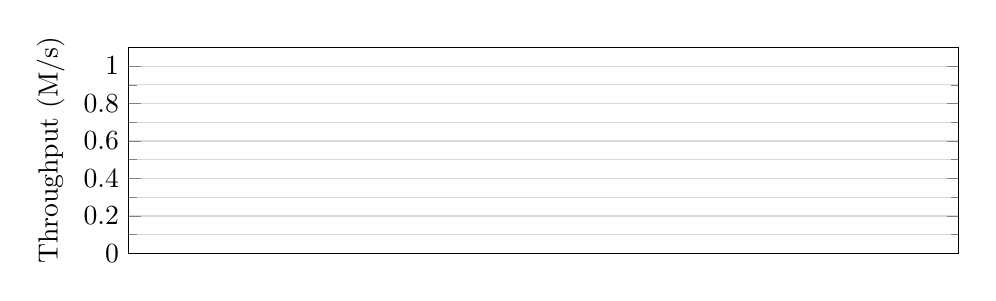
\begin{tikzpicture}
    \begin{axis}[
        width=\linewidth,
        height=4.2cm,
        ylabel={Throughput (M/s)},
        ylabel style={at={(ticklabel* cs:1.02)}, anchor=south},
        xlabel={},
        ybar,
        bar width=3pt,
        xtick={},
        xticklabels={},
        xtick style={draw=none},
        axis lines=box,
        tick align=inside,
        scaled ticks=true,
        tick label style={/pgf/number format/fixed,/pgf/number format/precision=1},
        ymajorgrids=true,
        yminorgrids=true,
        minor tick num=1,
        max space between ticks=35pt,
        try min ticks=5,
        grid style={gray!30},
        ymin=0,
        xmin=-8.75,
        xmax=16.5,
        legend entries = {\htthree, \htfour, \htfive, \htsix, \htone, \httwo},
        legend cell align = left,
        legend style={draw=none, legend columns=3, /tikz/every even column/.append style={column sep=0.3cm}},
        legend to name={intro-legend-horizontal}
    ]
    \addAllIntroLoadPlots
    \addAllIntroRunPlots

    % Add group labels
    \node at (axis cs:-3,375) {\text{Load}};
    \node at (axis cs:10.7,375) {\text{Run}};
    \end{axis}
    \end{tikzpicture}
    \caption{Throughput comparison on YCSB load and run phases.}\label{fig:intro_throughput}
    \end{subfigure}%
    \hfill
    % Subfigure (b): Space efficiency comparison
    \begin{subfigure}[t]{0.42\linewidth}
    \centering
    \begin{tikzpicture}
    \begin{axis}[
        width=\linewidth,
        height=4.2cm,
        ylabel={Space Efficiency (\%)},
        ylabel style={at={(ticklabel* cs:1.02)}, anchor=south},
        xlabel={},
        ybar,
        bar width=3pt,
        xticklabels={},
        xtick style={draw=none},
        axis lines=box,
        tick align=inside,
        scaled ticks=true,
        tick label style={/pgf/number format/fixed,/pgf/number format/precision=2},
        ymajorgrids=true,
        yminorgrids=true,
        minor tick num=1,
        max space between ticks=35pt,
        try min ticks=5,
        grid style={gray!30},
        ymin=0,
        xmin=-3,
        xmax=3
    ]

    % Space efficiency data (from max_space_efficiency.csv)
    \addAllSpaceEffPlots

    % Add invisible plot to extract the value for HTONE and display it
    \addplot[draw=none, fill=none, nodes near coords, point meta=explicit,
             nodes near coords style={font=\footnotesize}]
    table[x expr=-1, y expr=\thisrowno{1}*100-5, meta expr=\thisrowno{1}*100,
          restrict expr to domain={\thisrow{object_id}}{17:17}] {\maxspaceeffdata};

    \end{axis}
    \end{tikzpicture}
    \caption{Maximum space efficiency achieved in practice.}\label{fig:intro_space_efficiency}
    \end{subfigure}
    \caption{Performance comparison of \htabbr and state-of-the-art hash tables.}\label{fig:intro_figure}
\end{figure}


% Include YCSB plots

\begin{figure*}[h]
    \centering

    \pgfplotslegendfromname{throughput-legend-horizontal}

    % Single row: Load, Run A, Run B, Run C, Run A^-, Run B^-, Run C^-
    \generateSubfigure{17}{Load}{fill_throughput}{0}%
    \generateSubfigureNoYLabel{17}{Run A}{run_throughput}{0}%
    \generateSubfigureNoYLabel{18}{Run B}{run_throughput}{0}%
    \generateSubfigureNoYLabel{19}{Run C}{run_throughput}{0}%
    \generateSubfigureNoYLabel{20}{Run A$^-$}{run_throughput}{0}%
    \generateSubfigureNoYLabel{21}{Run B$^-$}{run_throughput}{0}%
    \generateSubfigureNoYLabel{22}{Run C$^-$}{run_throughput}{0}%
    \generateSubfigureNoYLabel{28}{Run X}{run_throughput}{0}

    \caption{Performance of hash tables on YCSB workloads with 16 threads. (Throughput is Million ops/second) \alex{I think this plot would be better if everything were on the same axis. It would also take up less space.}}\label{fig:throughput_subfigures}
\end{figure*}


% Include YCSB resizing plots
\begin{figure}[h]
    \centering
    \pgfplotslegendfromname{throughput-legend-3column}
    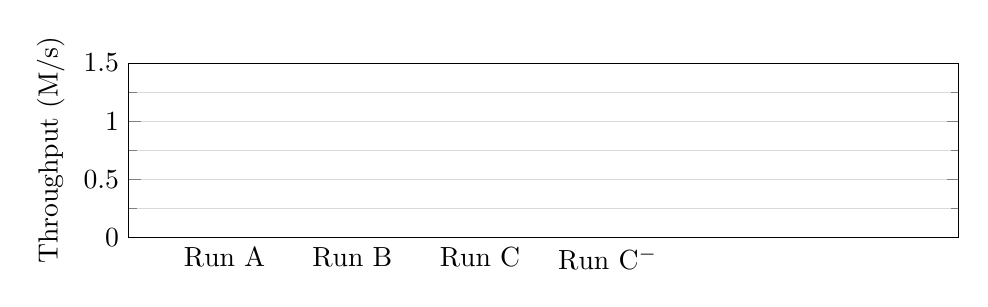
\begin{tikzpicture}
        \begin{axis}[
                width=\linewidth,
                height=3.8cm,
                ylabel={Throughput (M/s)},
                ybar,
                bar width=3pt,
                % enlarge x limits=0.12,
                enlarge x limits=0.15,
                % Use numeric x, but show your symbolic labels:
                xtick={0,1,2,3,4},
                xticklabels={Load,{Run A},{Run B},{Run C},{Run C$^-$}},
                % symbolic x coords={Load, {Run A}, {Run B}, {Run C}, {Run C$^-$}},
                axis lines=box,
                tick align=inside,
                xtick style={draw=none},
                scaled ticks=true,
                tick label style={/pgf/number format/fixed,/pgf/number format/precision=1},
                ymajorgrids=true,
                yminorgrids=true,
                minor tick num=1,
                max space between ticks=35pt,
                try min ticks=5,
                grid style={gray!30},
                enlarge y limits={upper,value=0.5},
                ymin=0,
                nodes near coords,
                nodes near coords align={vertical},
                nodes near coords style={font=\tiny, rotate=90, anchor=west, yshift=0.5pt, xshift=0.3pt},
                legend entries = {\htthree, \htfour, \htfive, \htsix, \htone, \httwo},
                legend cell align = left,
                legend style={draw=none, legend columns=3, /tikz/every even column/.append style={column sep=1cm}},
                legend to name={throughput-legend-3column},
                unbounded coords=discard,
                filter discard warning=false,
            ]

            \addResizingPlots

        \end{axis}
    \end{tikzpicture}

    \caption{Performance of hash tables on YCSB workloads with 16 threads (resizing enabled).}\label{fig:throughput_subfigures_resizing}
\end{figure}


% (Occupancy plots removed)

% Include throughput vs space efficiency plots

% Local helper: add all object plots for a given case_id
% #1 = case_id
\newcommand{\AddAllObjectPlotsForCase}[1]{%
    % \htthree (object_id=6)
    \addplot[CuckooLineStyle] table[
            x=space_efficiency,
            y=throughput_millions,
            restrict expr to domain={\thisrow{object_id}}{6:6},
            restrict expr to domain={\thisrow{case_id}}{#1:#1}
        ] {\throughputdata};

    % \htfour (object_id=7)
    \addplot[IcebergLineStyle] table[
            x=space_efficiency,
            y=throughput_millions,
            restrict expr to domain={\thisrow{object_id}}{7:7},
            restrict expr to domain={\thisrow{case_id}}{#1:#1}
        ] {\throughputdata};

    % \htfive (object_id=15)
    \addplot[JunctionLineStyle] table[
            x=space_efficiency,
            y=throughput_millions,
            restrict expr to domain={\thisrow{object_id}}{15:15},
            restrict expr to domain={\thisrow{case_id}}{#1:#1}
        ] {\throughputdata};

    % \htsix (object_id=24)
    \addplot[TBBLineStyle] table[
            x=space_efficiency,
            y=throughput_millions,
            restrict expr to domain={\thisrow{object_id}}{24:24},
            restrict expr to domain={\thisrow{case_id}}{#1:#1}
        ] {\throughputdata};

    % \htone (object_id=17)
    \addplot[TPHTLineStyle] table[
            x=space_efficiency,
            y=throughput_millions,
            restrict expr to domain={\thisrow{object_id}}{17:17},
            restrict expr to domain={\thisrow{case_id}}{#1:#1}
        ] {\throughputdata};

    % \httwo (object_id=23)
    \addplot[BlastLineStyle] table[
            x=space_efficiency,
            y=throughput_millions,
            restrict expr to domain={\thisrow{object_id}}{23:23},
            restrict expr to domain={\thisrow{case_id}}{#1:#1}
        ] {\throughputdata};
}

% Common axis style for all space efficiency plots
\pgfplotsset{
    spaceeff axis/.style={
            width=6.2cm,
            height=3.7cm,
            xlabel={Space Efficiency},
            xmin=0,
            ymin=0,
            grid=major,
            grid style={gray!30},
            tick label style={font=\small},
            label style={font=\small},
            scaled ticks=true,
            tick label style={/pgf/number format/fixed,/pgf/number format/precision=2},
            xtick distance=0.2,
            % ytick distance=10,
            minor tick num=1
        },
    spaceeff axis with ylabel/.style={
            spaceeff axis,
            ylabel={Throughput (M/s)}
        }
}

% Helper: create a subplot for a given case
% #1 = case_id, #2 = position (e.g., [b]{0.45\textwidth}), #3 = extra options for legend
\newcommand{\CreateSpaceEffSubplot}[3]{%
    \begin{subfigure}#2
        \centering
        \begin{tikzpicture}
            \begin{axis}[spaceeff axis, #3]
                \AddAllObjectPlotsForCase{#1}
            \end{axis}
        \end{tikzpicture}
        \caption{Case #1}
    \end{subfigure}%
}

\begin{figure*}[h]
    \centering
    \begin{minipage}{0.95\linewidth}
        \centering

        % Legend above figures in 1x5 layout
        {\pgfplotslegendfromname{spaceeff-legend}}

        % \vspace{0.5cm}

        % Case 1 with legend definition and y-label
        \begin{subfigure}[b]{0.35\textwidth}
            \centering
            \begin{tikzpicture}
                \begin{axis}[spaceeff axis with ylabel, legend to name={spaceeff-legend}, legend entries={\htthree, \htfour, \htfive, \htsix, \htone, \httwo}, legend cell align=left, legend style={draw=none, legend columns=6, /tikz/every even column/.append style={column sep=0.5cm}}]
                    \AddAllObjectPlotsForCase{1}
                \end{axis}
            \end{tikzpicture}
            \caption{Insertion}\label{fig:throughput_space_efficiency/insertion}
        \end{subfigure}%
        % Case 9 (no y-label)
        \begin{subfigure}[b]{0.32\textwidth}
            \centering
            \begin{tikzpicture}
                \begin{axis}[spaceeff axis]
                    \AddAllObjectPlotsForCase{9}
                \end{axis}
            \end{tikzpicture}
            \caption{Positive Query}\label{fig:throughput_space_efficiency/positive_query}
        \end{subfigure}%
        % Case 10 (no y-label)
        \begin{subfigure}[b]{0.32\textwidth}
            \centering
            \begin{tikzpicture}
                \begin{axis}[spaceeff axis]
                    \AddAllObjectPlotsForCase{10}
                \end{axis}
            \end{tikzpicture}
            \caption{Negative Query}\label{fig:throughput_space_efficiency/negative_query}
        \end{subfigure}
    \end{minipage}

    \caption{Throughput-space efficiency tradeoff across insertion and query workloads. Each curve shows how throughput and space efficiency vary with load factor, with rightmost points indicating maximum achievable space efficiency.}\label{fig:throughput_space_efficiency_cases}
\end{figure*}

% Include mem growth plots
% Mem growth plot: reads csv/mem_growth.csv and plots normalized time vs memory
\begin{figure}[h]
    \centering
    % Ensure the CSV path matches scripts/to_csv.sh output
    \pgfplotstableread[col sep=comma]{csv/mem_growth.csv}{\memgrowth}

    \begin{tikzpicture}
    \begin{axis}[
        width=8.5cm,
        height=6.0cm,
        xlabel={Normalized Time},
        ylabel={Memory Usage (MB)},
        xmin=0, xmax=1,
        grid=both,
        grid style={gray!30},
        legend style={draw=none, at={(0.5,1.02)}, anchor=south, legend columns=3, legend cell align=left},
        tick label style={font=\small},
        label style={font=\small}
    ]

    % List of object ids to plot; adjust if needed
    % Each line filters rows by object_id and plots as a line
    
    % Object 6 = Cuckoo (htthree)
    \addplot[CuckooLineStyle, mark=none]
        table[x=normalized_time, y=memory_mb, restrict expr to domain={\thisrow{object_id}}{6:6}] {\memgrowth};
    \addlegendentry{\htthree}

    % Object 7 = IcebergHT (htfour)
    \addplot[IcebergLineStyle, mark=none]
        table[x=normalized_time, y=memory_mb, restrict expr to domain={\thisrow{object_id}}{7:7}] {\memgrowth};
    \addlegendentry{\htfour}

    % Object 15 = Junction (htfive)
    \addplot[JunctionLineStyle, mark=none]
        table[x=normalized_time, y=memory_mb, restrict expr to domain={\thisrow{object_id}}{15:15}] {\memgrowth};
    \addlegendentry{\htfive}

    % Object 24 = TBB (htsix)
    \addplot[TBBLineStyle, mark=none]
        table[x=normalized_time, y=memory_mb, restrict expr to domain={\thisrow{object_id}}{24:24}] {\memgrowth};
    \addlegendentry{\htsix}

    % Object 18 = Chained-TPHT (htone)
    \addplot[TPHTLineStyle, mark=none]
        table[x=normalized_time, y=memory_mb, restrict expr to domain={\thisrow{object_id}}{18:18}] {\memgrowth};
    \addlegendentry{\htone}

    % Object 21 = Flattened-TPHT (httwo)
    \addplot[BlastLineStyle, mark=none]
        table[x=normalized_time, y=memory_mb, restrict expr to domain={\thisrow{object_id}}{21:21}] {\memgrowth};
    \addlegendentry{\httwo}

    \end{axis}
    \end{tikzpicture}

    \caption{Memory growth over normalized time across methods.}
    \label{fig:mem_growth_plot}
\end{figure}




% Include scaling plots
% Function to map case numbers to descriptive names
\newcommand{\getCaseName}[1]{%
    \ifnum#1=1 Insertion\fi%
    \ifnum#1=3 Deletion\fi%
    \ifnum#1=9 Positive Query\fi%
    \ifnum#1=10 Negative Query\fi%
}

% Helper macro to plot all objects for a given case
\newcommand{\AddAllObjectPlotsForScaling}[1]{%
    % \htthree (object_id=6)
    \addplot[CuckooLineStyle] table[
        x=thread_num,
        y expr=\thisrow{throughput (ops/s)}/1000000,
        restrict expr to domain={\thisrow{case_id}}{#1:#1},
        restrict expr to domain={\thisrow{object_id}}{6:6},
        restrict expr to domain={\thisrow{thread_num}}{0:17}
    ] {\scalingdata};
    
    % \htfour (object_id=7)
    \addplot[IcebergLineStyle] table[
        x=thread_num,
        y expr=\thisrow{throughput (ops/s)}/1000000,
        restrict expr to domain={\thisrow{case_id}}{#1:#1},
        restrict expr to domain={\thisrow{object_id}}{7:7},
        restrict expr to domain={\thisrow{thread_num}}{0:17}
    ] {\scalingdata};
    
    % \htfive (object_id=15)
    \addplot[JunctionLineStyle] table[
        x=thread_num,
        y expr=\thisrow{throughput (ops/s)}/1000000,
        restrict expr to domain={\thisrow{case_id}}{#1:#1},
        restrict expr to domain={\thisrow{object_id}}{15:15},
        restrict expr to domain={\thisrow{thread_num}}{0:17}
    ] {\scalingdata};
    
    % \htsix (object_id=24)
    \addplot[TBBLineStyle] table[
        x=thread_num,
        y expr=\thisrow{throughput (ops/s)}/1000000,
        restrict expr to domain={\thisrow{case_id}}{#1:#1},
        restrict expr to domain={\thisrow{object_id}}{24:24},
        restrict expr to domain={\thisrow{thread_num}}{0:17}
    ] {\scalingdata};
    
    % \htone (object_id=17)
    \addplot[TPHTLineStyle] table[
        x=thread_num,
        y expr=\thisrow{throughput (ops/s)}/1000000,
        restrict expr to domain={\thisrow{case_id}}{#1:#1},
        restrict expr to domain={\thisrow{object_id}}{17:17},
        restrict expr to domain={\thisrow{thread_num}}{0:17}
    ] {\scalingdata};
    
    % \httwo (object_id=20)
    \addplot[BlastLineStyle] table[
        x=thread_num,
        y expr=\thisrow{throughput (ops/s)}/1000000,
        restrict expr to domain={\thisrow{case_id}}{#1:#1},
        restrict expr to domain={\thisrow{object_id}}{20:20},
        restrict expr to domain={\thisrow{thread_num}}{0:17}
    ] {\scalingdata};
}


\begin{figure*}[h]
    \centering
    % Display shared legend
    {\pgfplotslegendfromname{spaceeff-legend}}
    % Case 1
    \begin{subfigure}[b]{0.27\textwidth}
        \centering
        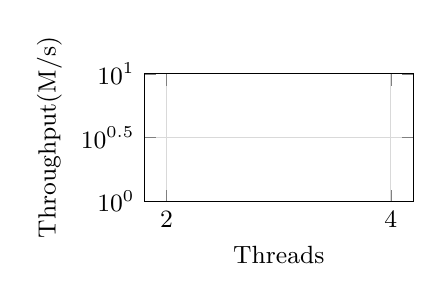
\begin{tikzpicture}
            \begin{axis}[
                    width=5cm,
                    height=3.2cm,
                    xlabel={Threads},
                    ylabel={Throughput(M/s)},
                    xmode=log,
                    ymode=log,
                    log basis x=2,
                    log basis y=10,
                    % xmin=0,
                    % xmax=20,
                    ymin=1,
                    ymax=400,
                    xtick={1,2,4,8,16},
                    xticklabels={1,2,4,8,16},
                    ytick={0.1,1,10,100},
                    grid=major,
                    grid style={gray!30},
                    tick label style={font=\small},
                    label style={font=\small},
                    % title={\getCaseName{1}},
                    % title style={font=\small},
                    scaled ticks=true,
                    tick label style={/pgf/number format/fixed,/pgf/number format/precision=1}
                ]

                \AddAllObjectPlotsForScaling{1}

            \end{axis}
        \end{tikzpicture}
        \caption{\getCaseName{1}}
    \end{subfigure}%
    % Case 3
    \begin{subfigure}[b]{0.24\textwidth}
        \centering
        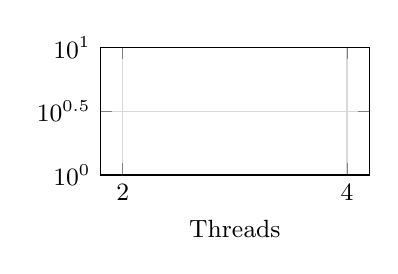
\begin{tikzpicture}
            \begin{axis}[
                    width=5cm,
                    height=3.2cm,
                    xlabel={Threads},
                    % ylabel={Throughput(M/s)},
                    xmode=log,
                    ymode=log,
                    log basis x=2,
                    log basis y=10,
                    % xmin=0,
                    % xmax=20,
                    ymin=1,
                    ymax=1000,
                    xtick={1,2,4,8,16},
                    xticklabels={1,2,4,8,16},
                    ytick={0.1,1,10,100,1000},
                    grid=major,
                    grid style={gray!30},
                    tick label style={font=\small},
                    label style={font=\small},
                    % title={\getCaseName{3}},
                    % title style={font=\small},
                    scaled ticks=true,
                    tick label style={/pgf/number format/fixed,/pgf/number format/precision=1}
                ]

                \AddAllObjectPlotsForScaling{3}

            \end{axis}
        \end{tikzpicture}
        \caption{\getCaseName{3}}
    \end{subfigure}%
    % Case 6
    \begin{subfigure}[b]{0.24\textwidth}
        \centering
        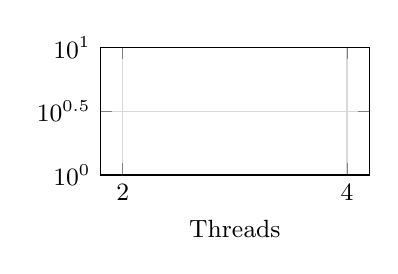
\begin{tikzpicture}
            \begin{axis}[
                    width=5cm,
                    height=3.2cm,
                    xlabel={Threads},
                    % ylabel={Throughput(M/s)},
                    xmode=log,
                    ymode=log,
                    log basis x=2,
                    log basis y=10,
                    % xmin=0,
                    % xmax=20,
                    ymin=1,
                    ymax=1000,
                    xtick={1,2,4,8,16},
                    xticklabels={1,2,4,8,16},
                    ytick={0.1,1,10,100,1000},
                    grid=major,
                    grid style={gray!30},
                    tick label style={font=\small},
                    label style={font=\small},
                    % title={\getCaseName{6}},
                    % title style={font=\small},
                    scaled ticks=true,
                    tick label style={/pgf/number format/fixed,/pgf/number format/precision=1}
                ]
                \AddAllObjectPlotsForScaling{9}
            \end{axis}
        \end{tikzpicture}
        \caption{\getCaseName{9}}
    \end{subfigure}%
    % Case 7
    \begin{subfigure}[b]{0.24\textwidth}
        \centering
        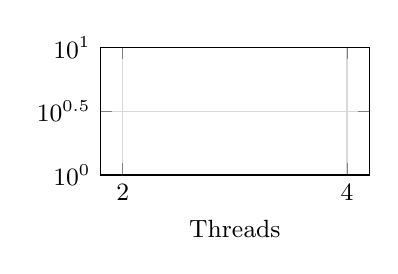
\begin{tikzpicture}
            \begin{axis}[
                    width=5cm,
                    height=3.2cm,
                    xlabel={Threads},
                    % ylabel={Throughput(M/s)},
                    xmode=log,
                    ymode=log,
                    log basis x=2,
                    log basis y=10,
                    % xmin=0,
                    % xmax=20,
                    ymin=1,
                    ymax=1000,
                    xtick={1,2,4,8,16},
                    xticklabels={1,2,4,8,16},
                    ytick={0.1,1,10,100,1000},
                    grid=major,
                    grid style={gray!30},
                    tick label style={font=\small},
                    label style={font=\small},
                    % title={\getCaseName{7}},
                    % title style={font=\small},
                    scaled ticks=true,
                    tick label style={/pgf/number format/fixed,/pgf/number format/precision=1}
                ]

                \AddAllObjectPlotsForScaling{10}

            \end{axis}
        \end{tikzpicture}
        \caption{\getCaseName{10}}
    \end{subfigure}%
    \caption{Performance scaling analysis for hash tables with increasing number of threads for 64M insertions.}\label{fig:scaling_analysis}
\end{figure*}

% Include prob analysis plots

\noindent
\begin{minipage}[t]{0.48\linewidth}
    \centering

    % Left: Load Factor (blue) with shading and markers
    \begin{tikzpicture}
        \begin{axis}[
                width=\linewidth,
                height=4cm,
                xlabel={Bin Size},
                ylabel={Load Factor Support (\%)},
                xmode=log,
                xmin=2,
                xmax=190,
                ymin=0,
                ymax=105,
                ytick={0,20,40,60,80,100},
                grid=major,
                grid style={gray!30},
                % clip=false,
                legend style={draw=none, font=\footnotesize, at={(0.5,1.02)}, anchor=south},
                legend columns=1,
                tick label style={font=\small},
                label style={font=\small},
                scaled ticks=true,
                xtick={3,7,15,31,63,127},
                xticklabels={$2^2$,$2^3$,$2^4$,$2^5$,$2^6$,$2^7$}
            ]

            % Legend entries
            \addlegendimage{InsertionOnlyStyle, mark=o, mark size=2.5pt}
            \addlegendentry{Insertion Only}
            \addlegendimage{WithDeletionStyle, mark=square, mark size=2.5pt}
            \addlegendentry{With Deletion}

            % Insertion (CSV) shaded area and line with markers
            \addplot[name path=insLineMini, draw=none] table[
                    x=bin_size,
                    y index=3,
                    col sep=comma,
                    restrict expr to domain={\thisrow{object_id}}{4:4}
                ] {\loadfactordata};
            \addplot[name path=insBaseMini, draw=none] coordinates {(3,0) (127,0)};
            \addplot[fill=exp1!25, fill opacity=0.35, draw=none, forget plot] fill between[of=insLineMini and insBaseMini];
            \addplot[InsertionOnlyStyle, mark=o, mark size=2.5pt] table[
                    x=bin_size,
                    y index=3,
                    col sep=comma,
                    restrict expr to domain={\thisrow{object_id}}{4:4}
                ] {\loadfactordata};

            % Deletion (hardcoded) shaded area and line with markers
            \addplot[name path=delLineMini, draw=none] coordinates {
                    (3,7)
                    (7,43)
                    (15,71)
                    (31,85)
                    (63,91)
                    (127,95)
                };
            \addplot[name path=delBaseMini, draw=none] coordinates {(3,0) (127,0)};
            \addplot[fill=poisson!25, fill opacity=0.35, draw=none, forget plot] fill between[of=delLineMini and delBaseMini];
            \addplot[WithDeletionStyle, mark=square, mark size=2.5pt] coordinates {
                    (3,7)
                    (7,43)
                    (15,71)
                    (31,85)
                    (63,91)
                    (127,95)
                };
        \end{axis}
    \end{tikzpicture}

    \captionof{figure}{Load factor supported by dereference tables across bin sizes (Section~\ref{subsec:tpimpl}).}\label{fig:prob_load_mini}
\end{minipage}%
\hfill%
\begin{minipage}[t]{0.48\linewidth}
    \centering

    % Right: Occupancy (log scale) with boxplots and shaded Poisson
    \begin{tikzpicture}
        \begin{axis}[
                width=\linewidth,
                height=4cm,
                xlabel={Bin Occupancy},
                ylabel={Relative Frequency},
                ymode=log,
                ymin=1e-9,
                ymax=2.5,
                ytick={1e-1, 1e-3, 1e-5, 1e-7, 1e-9},
                xmin=0,
                xmax=11.5,
                xtick={0,1,3,5,7,9,11},
                xticklabels={0,1,3,5,7,9,11},
                grid=major,
                grid style={gray!30},
                % clip=false,
                legend style={draw=none, font=\footnotesize, at={(0.4,1.02)}, anchor=south, legend image post style={scale=0.5}},
                legend columns=2,
                legend cell align=left,
                tick label style={font=\small},
                label style={font=\small}
            ]

            % Legend entries
            \addlegendimage{area legend, draw=exp1, fill=exp1!25}
            \addlegendentry{Random}
            \addlegendimage{area legend, draw=exp2, fill=exp2!25}
            \addlegendentry{Sequential}
            \addlegendimage{area legend, draw=exp3, fill=exp3!25}
            \addlegendentry{Low Hamming}
            \addlegendimage{area legend, draw=exp4, fill=exp4!25}
            \addlegendentry{High Hamming}
            \addlegendimage{PoissonTheoryStyle}
            \addlegendentry{Poisson ($\lambda=1$)}

            % Box plots 0..11 with all key sets
            \foreach \i in {0,1,2,3,4,5,6,7,8,9,10,11} {
                % Random keys (leftmost)
                \pgfplotstablegetelem{\i}{lower_whisker}\of{\occboxrandom}\edef\lw{\pgfplotsretval}
                \pgfplotstablegetelem{\i}{lower}\of{\occboxrandom}\edef\lq{\pgfplotsretval}
                \pgfplotstablegetelem{\i}{median}\of{\occboxrandom}\edef\med{\pgfplotsretval}
                \pgfplotstablegetelem{\i}{upper}\of{\occboxrandom}\edef\uq{\pgfplotsretval}
                \pgfplotstablegetelem{\i}{upper_whisker}\of{\occboxrandom}\edef\uw{\pgfplotsretval}
                \pgfmathsetmacro{\pos}{\i - 0.3}
                \edef\boxopts{boxplot prepared={draw position=\pos, lower whisker=\lw, lower quartile=\lq, median=\med, upper quartile=\uq, upper whisker=\uw}, boxplot/draw direction=y, fill=exp1!25, draw=exp1}
                \expandafter\addplot\expandafter+\expandafter[\boxopts] coordinates {};
                
                % Sequential keys
                \pgfplotstablegetelem{\i}{lower_whisker}\of{\occboxsequential}\edef\lw{\pgfplotsretval}
                \pgfplotstablegetelem{\i}{lower}\of{\occboxsequential}\edef\lq{\pgfplotsretval}
                \pgfplotstablegetelem{\i}{median}\of{\occboxsequential}\edef\med{\pgfplotsretval}
                \pgfplotstablegetelem{\i}{upper}\of{\occboxsequential}\edef\uq{\pgfplotsretval}
                \pgfplotstablegetelem{\i}{upper_whisker}\of{\occboxsequential}\edef\uw{\pgfplotsretval}
                \pgfmathsetmacro{\pos}{\i - 0.1}
                \edef\boxopts{boxplot prepared={draw position=\pos, lower whisker=\lw, lower quartile=\lq, median=\med, upper quartile=\uq, upper whisker=\uw}, boxplot/draw direction=y, fill=exp2!25, draw=exp2, very thick}
                \expandafter\addplot\expandafter+\expandafter[\boxopts] coordinates {};
                
                % Low Hamming keys
                \pgfplotstablegetelem{\i}{lower_whisker}\of{\occboxlowhamming}\edef\lw{\pgfplotsretval}
                \pgfplotstablegetelem{\i}{lower}\of{\occboxlowhamming}\edef\lq{\pgfplotsretval}
                \pgfplotstablegetelem{\i}{median}\of{\occboxlowhamming}\edef\med{\pgfplotsretval}
                \pgfplotstablegetelem{\i}{upper}\of{\occboxlowhamming}\edef\uq{\pgfplotsretval}
                \pgfplotstablegetelem{\i}{upper_whisker}\of{\occboxlowhamming}\edef\uw{\pgfplotsretval}
                \pgfmathsetmacro{\pos}{\i + 0.1}
                \edef\boxopts{boxplot prepared={draw position=\pos, lower whisker=\lw, lower quartile=\lq, median=\med, upper quartile=\uq, upper whisker=\uw}, boxplot/draw direction=y, fill=exp3!25, draw=exp3}
                \expandafter\addplot\expandafter+\expandafter[\boxopts] coordinates {};
                
                % High Hamming keys (rightmost)
                \pgfplotstablegetelem{\i}{lower_whisker}\of{\occboxhighhamming}\edef\lw{\pgfplotsretval}
                \pgfplotstablegetelem{\i}{lower}\of{\occboxhighhamming}\edef\lq{\pgfplotsretval}
                \pgfplotstablegetelem{\i}{median}\of{\occboxhighhamming}\edef\med{\pgfplotsretval}
                \pgfplotstablegetelem{\i}{upper}\of{\occboxhighhamming}\edef\uq{\pgfplotsretval}
                \pgfplotstablegetelem{\i}{upper_whisker}\of{\occboxhighhamming}\edef\uw{\pgfplotsretval}
                \pgfmathsetmacro{\pos}{\i + 0.3}
                \edef\boxopts{boxplot prepared={draw position=\pos, lower whisker=\lw, lower quartile=\lq, median=\med, upper quartile=\uq, upper whisker=\uw}, boxplot/draw direction=y, fill=exp4!25, draw=exp4}
                \expandafter\addplot\expandafter+\expandafter[\boxopts] coordinates {};
            }

            % Shaded Poisson under curve and line on top
            \addplot[fill=poisson!25, fill opacity=0.35, draw=none, forget plot] table[
                    x=x,
                    y=y
                ] {\occpois} |- (axis cs:10,1.1e-9) -- (axis cs:0,1.1e-9) -- cycle;
            \addplot[PoissonTheoryStyle, mark=none] table[
                    x=x,
                    y=y
                ] {\occpois};
        \end{axis}
    \end{tikzpicture}

    \captionof{figure}{Bin occupancy compared with smoothed Poisson ($\lambda=1$).}\label{fig:prob_occ_mini}
\end{minipage}


% Include load factor support plots

\begin{figure}[p]
    \centering
    \pgfplotslegendfromname{lflegend}
    
    \begin{tikzpicture}
        \begin{axis}[
            width=12cm,
            height=8cm,
            xlabel={Bin Size},
            ylabel={Load Factor Support (\%)},
            xmode=log,
            xmin=2,
            xmax=190,
            ymin=0,
            ymax=105,
            grid=major,
            grid style={gray!30},
            legend to name=lflegend,
            legend columns=1,
            legend style={draw=none, font=\small},
            tick label style={font=\small},
            label style={font=\small},
            scaled ticks=true,
            xtick={3,7,15,31,63,127},
            xticklabels={$2^2$,$2^3$,$2^4$,$2^5$,$2^6$,$2^7$}
        ]

        % Plot insertion data (from CSV) - blue with shade and markers
        \addplot[name path=insLine, draw=none, InsertionOnlyStyle] table[
            x=bin_size,
            y index=3,
            col sep=comma,
            restrict expr to domain={\thisrow{object_id}}{4:4}
        ] {\loadfactordata};
        \addlegendentry{Insertion Only}
        \addplot[name path=insBase, draw=none] coordinates {(3,0) (127,0)};
        \addplot[fill=exp1!25, fill opacity=0.35, draw=none, forget plot] fill between[of=insLine and insBase];
        \addplot[InsertionOnlyStyle, mark=o, mark size=2.5pt] table[
            x=bin_size,
            y index=3,
            col sep=comma,
            restrict expr to domain={\thisrow{object_id}}{4:4}
        ] {\loadfactordata};

        % Plot deletion data (hardcoded) - purple with shade and markers
        \addplot[name path=delLine, draw=none, WithDeletionStyle] coordinates {
            (3,7)
            (7,43)
            (15,71)
            (31,85)
            (63,91)
            (127,95)
        };
        \addlegendentry{With Deletion}
        \addplot[name path=delBase, draw=none] coordinates {(3,0) (127,0)};
        \addplot[fill=poisson!25, fill opacity=0.35, draw=none, forget plot] fill between[of=delLine and delBase];
        \addplot[WithDeletionStyle, mark=square*, mark size=2.5pt] coordinates {
            (3,7)
            (7,43)
            (15,71)
            (31,85)
            (63,91)
            (127,95)
        };

        \end{axis}
    \end{tikzpicture}
    \caption{Load Factor Support vs Bin Size for different hash table implementations. The x-axis shows bin size on a logarithmic scale, while the y-axis shows the maximum supported load factor as a percentage.}\label{fig:load_factor_support}
\end{figure} 


\begin{figure}[p]
    \centering
    \pgfplotslegendfromname{occlegend}

    % Box plot style occupancy distribution
    \begin{subfigure}[b]{0.48\textwidth}
        \centering
        \begin{tikzpicture}
            \begin{axis}[
                    width=8cm,
                    height=7cm,
                    xlabel={Number of Balls per Bin},
                    ylabel={Probability (Log Scale)},
                    ymode=log,
                    ymin=1e-9,
                    ymax=2,
                    xmin=-0.5,
                    xmax=11.5,
                    xtick={0,1,2,3,4,5,6,7,8,9,10,11},
                    xticklabels={0,1,2,3,4,5,6,7,8,9,10,11},
                    grid=major,
                    grid style={gray!30},
                    legend to name=occlegend,
                    legend columns=1,
                    legend style={draw=none, font=\small},
                    tick label style={font=\small},
                    label style={font=\small}
                ]

                % Unified legend symbols (exported to figure-level legend)
                \addlegendimage{area legend, draw=exp1, fill=exp1!25}
                \addlegendentry{Random Keys}
                \addlegendimage{area legend, draw=exp2, fill=exp2!25}
                \addlegendentry{Sequential Keys}
                \addlegendimage{area legend, draw=exp3, fill=exp3!25}
                \addlegendentry{Low Hamming Keys}
                \addlegendimage{area legend, draw=exp4, fill=exp4!25}
                \addlegendentry{High Hamming Keys}
                \addlegendimage{PoissonTheoryStyle}
                \addlegendentry{Poisson Theory ($\lambda=1$)}

                % Box plots for occupancy 0-11 with all key sets
                \foreach \i in {0,1,2,3,4,5,6,7,8,9,10,11} {
                        % Random keys (leftmost)
                        \pgfplotstablegetelem{\i}{lower_whisker}\of{\occboxrandom}\edef\lw{\pgfplotsretval}
                        \pgfplotstablegetelem{\i}{lower}\of{\occboxrandom}\edef\lq{\pgfplotsretval}
                        \pgfplotstablegetelem{\i}{median}\of{\occboxrandom}\edef\med{\pgfplotsretval}
                        \pgfplotstablegetelem{\i}{upper}\of{\occboxrandom}\edef\uq{\pgfplotsretval}
                        \pgfplotstablegetelem{\i}{upper_whisker}\of{\occboxrandom}\edef\uw{\pgfplotsretval}
                        \pgfmathsetmacro{\pos}{\i - 0.3}
                        \edef\boxopts{boxplot prepared={draw position=\pos, lower whisker=\lw, lower quartile=\lq, median=\med, upper quartile=\uq, upper whisker=\uw}, boxplot/draw direction=y, fill=exp1!25, draw=exp1}
                        \expandafter\addplot\expandafter+\expandafter[\boxopts] coordinates {};
                        
                        % Sequential keys
                        \pgfplotstablegetelem{\i}{lower_whisker}\of{\occboxsequential}\edef\lw{\pgfplotsretval}
                        \pgfplotstablegetelem{\i}{lower}\of{\occboxsequential}\edef\lq{\pgfplotsretval}
                        \pgfplotstablegetelem{\i}{median}\of{\occboxsequential}\edef\med{\pgfplotsretval}
                        \pgfplotstablegetelem{\i}{upper}\of{\occboxsequential}\edef\uq{\pgfplotsretval}
                        \pgfplotstablegetelem{\i}{upper_whisker}\of{\occboxsequential}\edef\uw{\pgfplotsretval}
                        \pgfmathsetmacro{\pos}{\i - 0.1}
                        \edef\boxopts{boxplot prepared={draw position=\pos, lower whisker=\lw, lower quartile=\lq, median=\med, upper quartile=\uq, upper whisker=\uw}, boxplot/draw direction=y, fill=exp2!25, draw=exp2, very thick}
                        \expandafter\addplot\expandafter+\expandafter[\boxopts] coordinates {};
                        
                        % Low Hamming keys
                        \pgfplotstablegetelem{\i}{lower_whisker}\of{\occboxlowhamming}\edef\lw{\pgfplotsretval}
                        \pgfplotstablegetelem{\i}{lower}\of{\occboxlowhamming}\edef\lq{\pgfplotsretval}
                        \pgfplotstablegetelem{\i}{median}\of{\occboxlowhamming}\edef\med{\pgfplotsretval}
                        \pgfplotstablegetelem{\i}{upper}\of{\occboxlowhamming}\edef\uq{\pgfplotsretval}
                        \pgfplotstablegetelem{\i}{upper_whisker}\of{\occboxlowhamming}\edef\uw{\pgfplotsretval}
                        \pgfmathsetmacro{\pos}{\i + 0.1}
                        \edef\boxopts{boxplot prepared={draw position=\pos, lower whisker=\lw, lower quartile=\lq, median=\med, upper quartile=\uq, upper whisker=\uw}, boxplot/draw direction=y, fill=exp3!25, draw=exp3}
                        \expandafter\addplot\expandafter+\expandafter[\boxopts] coordinates {};
                        
                        % High Hamming keys (rightmost)
                        \pgfplotstablegetelem{\i}{lower_whisker}\of{\occboxhighhamming}\edef\lw{\pgfplotsretval}
                        \pgfplotstablegetelem{\i}{lower}\of{\occboxhighhamming}\edef\lq{\pgfplotsretval}
                        \pgfplotstablegetelem{\i}{median}\of{\occboxhighhamming}\edef\med{\pgfplotsretval}
                        \pgfplotstablegetelem{\i}{upper}\of{\occboxhighhamming}\edef\uq{\pgfplotsretval}
                        \pgfplotstablegetelem{\i}{upper_whisker}\of{\occboxhighhamming}\edef\uw{\pgfplotsretval}
                        \pgfmathsetmacro{\pos}{\i + 0.3}
                        \edef\boxopts{boxplot prepared={draw position=\pos, lower whisker=\lw, lower quartile=\lq, median=\med, upper quartile=\uq, upper whisker=\uw}, boxplot/draw direction=y, fill=exp4!25, draw=exp4}
                        \expandafter\addplot\expandafter+\expandafter[\boxopts] coordinates {};
                    }
                % Fill under Poisson line (log axis) by closing to baseline
                \addplot[fill=poisson!25, fill opacity=0.35, draw=none, forget plot] table[
                        x=x,
                        y=y
                    ] {\occpois} |- (axis cs:10,1.1e-9) -- (axis cs:0,1.1e-9) -- cycle;
                % Draw visible Poisson line on top
                \addplot[PoissonTheoryStyle, mark=none] table[
                        x=x,
                        y=y
                    ] {\occpois};
            \end{axis}
        \end{tikzpicture}
        \caption{Distribution Comparison (Log Scale)}
    \end{subfigure}
    \hfill
    % Linear scale for low occupancy values
    \begin{subfigure}[b]{0.48\textwidth}
        \centering
        \begin{tikzpicture}
            \begin{axis}[
                    width=8cm,
                    height=7cm,
                    xlabel={Number of Balls per Bin},
                    ylabel={Probability},
                    xmin=-0.5,
                    xmax=11.5,
                    ymin=0,
                    xtick={0,1,2,3,4,5,6,7,8,9,10,11},
                    xticklabels={0,1,2,3,4,5,6,7,8,9,10,11},
                    grid=major,
                    grid style={gray!30},
                    legend style={draw=none, font=\small},
                    tick label style={font=\small},
                    label style={font=\small}
                ]

                % Box plots for occupancy 0-5 with all key sets
                \foreach \i in {0,1,2,3,4,5} {
                        % Random keys (leftmost)
                        \pgfplotstablegetelem{\i}{lower_whisker}\of{\occboxrandom}\edef\lw{\pgfplotsretval}
                        \pgfplotstablegetelem{\i}{lower}\of{\occboxrandom}\edef\lq{\pgfplotsretval}
                        \pgfplotstablegetelem{\i}{median}\of{\occboxrandom}\edef\med{\pgfplotsretval}
                        \pgfplotstablegetelem{\i}{upper}\of{\occboxrandom}\edef\uq{\pgfplotsretval}
                        \pgfplotstablegetelem{\i}{upper_whisker}\of{\occboxrandom}\edef\uw{\pgfplotsretval}
                        \pgfmathsetmacro{\pos}{\i - 0.3}
                        \edef\boxopts{boxplot prepared={draw position=\pos, lower whisker=\lw, lower quartile=\lq, median=\med, upper quartile=\uq, upper whisker=\uw}, boxplot/draw direction=y, fill=exp1!25, draw=exp1}
                        \expandafter\addplot\expandafter+\expandafter[\boxopts] coordinates {};
                        
                        % Sequential keys
                        \pgfplotstablegetelem{\i}{lower_whisker}\of{\occboxsequential}\edef\lw{\pgfplotsretval}
                        \pgfplotstablegetelem{\i}{lower}\of{\occboxsequential}\edef\lq{\pgfplotsretval}
                        \pgfplotstablegetelem{\i}{median}\of{\occboxsequential}\edef\med{\pgfplotsretval}
                        \pgfplotstablegetelem{\i}{upper}\of{\occboxsequential}\edef\uq{\pgfplotsretval}
                        \pgfplotstablegetelem{\i}{upper_whisker}\of{\occboxsequential}\edef\uw{\pgfplotsretval}
                        \pgfmathsetmacro{\pos}{\i - 0.1}
                        \edef\boxopts{boxplot prepared={draw position=\pos, lower whisker=\lw, lower quartile=\lq, median=\med, upper quartile=\uq, upper whisker=\uw}, boxplot/draw direction=y, fill=exp2!25, draw=exp2, very thick}
                        \expandafter\addplot\expandafter+\expandafter[\boxopts] coordinates {};
                        
                        % Low Hamming keys
                        \pgfplotstablegetelem{\i}{lower_whisker}\of{\occboxlowhamming}\edef\lw{\pgfplotsretval}
                        \pgfplotstablegetelem{\i}{lower}\of{\occboxlowhamming}\edef\lq{\pgfplotsretval}
                        \pgfplotstablegetelem{\i}{median}\of{\occboxlowhamming}\edef\med{\pgfplotsretval}
                        \pgfplotstablegetelem{\i}{upper}\of{\occboxlowhamming}\edef\uq{\pgfplotsretval}
                        \pgfplotstablegetelem{\i}{upper_whisker}\of{\occboxlowhamming}\edef\uw{\pgfplotsretval}
                        \pgfmathsetmacro{\pos}{\i + 0.1}
                        \edef\boxopts{boxplot prepared={draw position=\pos, lower whisker=\lw, lower quartile=\lq, median=\med, upper quartile=\uq, upper whisker=\uw}, boxplot/draw direction=y, fill=exp3!25, draw=exp3}
                        \expandafter\addplot\expandafter+\expandafter[\boxopts] coordinates {};
                        
                        % High Hamming keys (rightmost)
                        \pgfplotstablegetelem{\i}{lower_whisker}\of{\occboxhighhamming}\edef\lw{\pgfplotsretval}
                        \pgfplotstablegetelem{\i}{lower}\of{\occboxhighhamming}\edef\lq{\pgfplotsretval}
                        \pgfplotstablegetelem{\i}{median}\of{\occboxhighhamming}\edef\med{\pgfplotsretval}
                        \pgfplotstablegetelem{\i}{upper}\of{\occboxhighhamming}\edef\uq{\pgfplotsretval}
                        \pgfplotstablegetelem{\i}{upper_whisker}\of{\occboxhighhamming}\edef\uw{\pgfplotsretval}
                        \pgfmathsetmacro{\pos}{\i + 0.3}
                        \edef\boxopts{boxplot prepared={draw position=\pos, lower whisker=\lw, lower quartile=\lq, median=\med, upper quartile=\uq, upper whisker=\uw}, boxplot/draw direction=y, fill=exp4!25, draw=exp4}
                        \expandafter\addplot\expandafter+\expandafter[\boxopts] coordinates {};
                    }

                % Fill under Poisson line (linear axis) by closing to baseline
                \addplot[fill=poisson!25, fill opacity=0.35, draw=none, forget plot] table[
                        x=x,
                        y=y,
                        restrict expr to domain={\thisrow{x}}{0:5}
                    ] {\occpois} |- (axis cs:5,0) -- (axis cs:0,0) -- cycle;
                \addplot[PoissonTheoryStyle, mark=none] table[
                        x=x,
                        y=y,
                        restrict expr to domain={\thisrow{x}}{0:5}
                    ] {\occpois};
            \end{axis}
        \end{tikzpicture}
        \caption{Common Values (Linear Scale)}
    \end{subfigure}

    \caption{Hash Function Occupancy Distribution Analysis for Different Key Sets. Left: Full distribution on logarithmic scale showing rare events. Right: Linear scale focusing on common occupancy values (0--5 balls). Box plots compare random, sequential, low Hamming distance, and high Hamming distance key sets against the theoretical Poisson distribution ($\lambda=1$).}\label{fig:occupancy_analysis}
\end{figure}


% Include data size scaling plots
% Helper to map case id to label
\newcommand{\getScalingCaseName}[1]{%
  \ifnum#1=1 Insertion\fi%
  \ifnum#1=3 Deletion\fi%
  \ifnum#1=9 Positive Query\fi%
  \ifnum#1=10 Negative Query\fi%
}

% Helper to add all 6 objects with consistent styles
\newcommand{\AddAllObjectsForDataSize}[1]{%
  % \htthree (6)
  \addplot[CuckooLineStyle] table[
      x=table_size,
      y expr=\thisrow{throughput (ops/s)}/1000000,
      restrict expr to domain={\thisrow{case_id}}{#1:#1},
      restrict expr to domain={\thisrow{object_id}}{6:6},
      restrict expr to domain={\thisrow{table_size}}{32768:1000000000}
    ] {\datasizedata};
  % \htfour (7)
  \addplot[IcebergLineStyle] table[
      x=table_size,
      y expr=\thisrow{throughput (ops/s)}/1000000,
      restrict expr to domain={\thisrow{case_id}}{#1:#1},
      restrict expr to domain={\thisrow{object_id}}{7:7},
      restrict expr to domain={\thisrow{table_size}}{32768:1000000000}
    ] {\datasizedata};
  % \htfive (15)
  \addplot[JunctionLineStyle] table[
      x=table_size,
      y expr=\thisrow{throughput (ops/s)}/1000000,
      restrict expr to domain={\thisrow{case_id}}{#1:#1},
      restrict expr to domain={\thisrow{object_id}}{15:15},
      restrict expr to domain={\thisrow{table_size}}{32768:1000000000}
    ] {\datasizedata};
  % \htsix (24)
  \addplot[TBBLineStyle] table[
      x=table_size,
      y expr=\thisrow{throughput (ops/s)}/1000000,
      restrict expr to domain={\thisrow{case_id}}{#1:#1},
      restrict expr to domain={\thisrow{object_id}}{24:24},
      restrict expr to domain={\thisrow{table_size}}{32768:1000000000}
    ] {\datasizedata};
  % \htone (17)
  \addplot[TPHTLineStyle] table[
      x=table_size,
      y expr=\thisrow{throughput (ops/s)}/1000000,
      restrict expr to domain={\thisrow{case_id}}{#1:#1},
      restrict expr to domain={\thisrow{object_id}}{17:17},
      restrict expr to domain={\thisrow{table_size}}{32768:1000000000}
    ] {\datasizedata};
  % \httwo (20)
  \addplot[BlastLineStyle] table[
      x=table_size,
      y expr=\thisrow{throughput (ops/s)}/1000000,
      restrict expr to domain={\thisrow{case_id}}{#1:#1},
      restrict expr to domain={\thisrow{object_id}}{20:20},
      restrict expr to domain={\thisrow{table_size}}{32768:1000000000}
    ] {\datasizedata};
}

% Shared legend (reuse scaling legend styles)
\begin{figure*}[h]
  \centering
  {\pgfplotslegendfromname{spaceeff-legend}}
  % Case 1
  \begin{subfigure}[b]{0.27\textwidth}
    \tiny
    \centering
    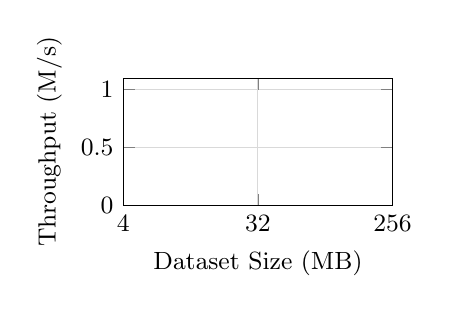
\begin{tikzpicture}
      \begin{axis}[
          width=5cm,
          height=3.2cm,
          xlabel={Dataset Size (MB)},
          ylabel={Throughput (M/s)},
          xmode=log,
          log basis x=2,
          ymin=0,
          xmin=131072,
          xmax=268435456,
          xtick={262144,2097152,16777216,134217728},
          xticklabels={4,32,256,2048},
          grid=major,
          grid style={gray!30},
          tick label style={font=\small},
          label style={font=\small},
          scaled ticks=true,
          tick label style={/pgf/number format/fixed,/pgf/number format/precision=1}
        ]
        \AddAllObjectsForDataSize{1}
      \end{axis}
    \end{tikzpicture}
    \caption{\getScalingCaseName{1}}
  \end{subfigure}%
  % Case 3
  \begin{subfigure}[b]{0.24\textwidth}
    \tiny
    \centering
    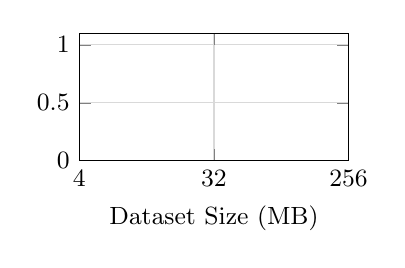
\begin{tikzpicture}
      \begin{axis}[
          width=5cm,
          height=3.2cm,
          xlabel={Dataset Size (MB)},
          % ylabel={Throughput (M/s)},
          xmode=log,
          log basis x=2,
          ymin=0,
          xmin=131072,
          xmax=268435456,
          xtick={262144,2097152,16777216,134217728},
          xticklabels={4,32,256,2048},
          grid=major,
          grid style={gray!30},
          tick label style={font=\small},
          label style={font=\small},
          scaled ticks=true,
          tick label style={/pgf/number format/fixed,/pgf/number format/precision=1}
        ]
        \AddAllObjectsForDataSize{3}
      \end{axis}
    \end{tikzpicture}
    \caption{\getScalingCaseName{3}}
  \end{subfigure}%
  % Case 6
  \begin{subfigure}[b]{0.24\textwidth}
    \tiny
    \centering
    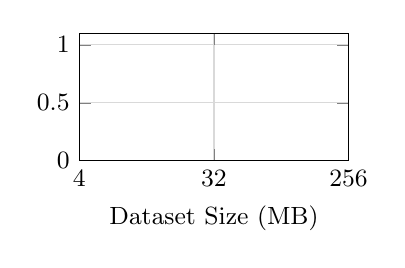
\begin{tikzpicture}
      \begin{axis}[
          width=5cm,
          height=3.2cm,
          xlabel={Dataset Size (MB)},
          % ylabel={Throughput (M/s)},
          xmode=log,
          log basis x=2,
          ymin=0,
          xmin=131072,
          xmax=268435456,
          xtick={262144,2097152,16777216,134217728},
          xticklabels={4,32,256,2048},
          grid=major,
          grid style={gray!30},
          tick label style={font=\small},
          label style={font=\small},
          scaled ticks=true,
          tick label style={/pgf/number format/fixed,/pgf/number format/precision=1}
        ]
        \AddAllObjectsForDataSize{9}
      \end{axis}
    \end{tikzpicture}
    \caption{\getScalingCaseName{9}}
  \end{subfigure}%
  % Case 7
  \begin{subfigure}[b]{0.24\textwidth}
    \tiny
    \centering
    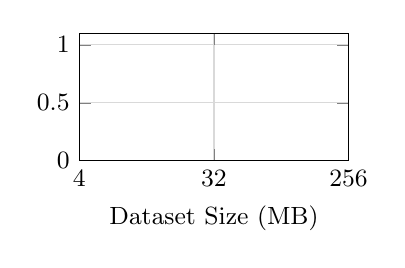
\begin{tikzpicture}
      \begin{axis}[
          width=5cm,
          height=3.2cm,
          xlabel={Dataset Size (MB)},
          % ylabel={Throughput (M/s)},
          xmode=log,
          log basis x=2,
          ymin=0,
          xmin=131072,
          xmax=268435456,
          xtick={262144,2097152,16777216,134217728},
          xticklabels={4,32,256,2048},
          grid=major,
          grid style={gray!30},
          tick label style={font=\small},
          label style={font=\small},
          scaled ticks=true,
          tick label style={/pgf/number format/fixed,/pgf/number format/precision=1}
        ]
        \AddAllObjectsForDataSize{10}
      \end{axis}
    \end{tikzpicture}
    \caption{\getScalingCaseName{10}}
  \end{subfigure}%
  \caption{Performance scaling analysis for hash tables with increasing dataset size, single-threaded.}\label{fig:data_size_scaling}
\end{figure*}

% Include percentile tables
\begin{table*}[t]
  \centering
  \tightsize
  \caption{Latency percentiles for insertion and positive query operations during resizing scenarios of YCSB Run A.}\label{tab:latency_percentiles}
  \begin{threeparttable}
  \footnotesize
  \begin{tabular}{l *{6}{r} *{6}{r}}
    \toprule
    & \multicolumn{6}{c}{\textbf{Insertion}} & \multicolumn{6}{c}{\textbf{Positive Query}} \\
    \cmidrule(lr){2-7}\cmidrule(lr){8-13}
    \textbf{Percentile} & \htthree & \htfour & \htfive & \htsix & \htone & \httwo
                        & \htthree & \htfour & \htfive & \htsix & \htone & \httwo \\
    \midrule
    \(50\%\)    & 200ns & 215ns & 423ns & 1.4$\mu$s & 346ns & 165ns & 167ns & 231ns & 142ns & 878ns & 277ns & 150ns \\
    \(95\%\)    & 989ns & 684ns & 37.0$\mu$s & 2.8$\mu$s & 606ns & 390ns & 384ns & 496ns & 717ns & 1.8$\mu$s & 545ns & 237ns \\
    \(99\%\)    & 2.7$\mu$s & 1.4$\mu$s & 66.4$\mu$s & 3.7$\mu$s & 788ns & 541ns & 565ns & 650ns & 1.4$\mu$s & 2.4$\mu$s & 710ns & 497ns \\
    \(99.9\%\)  & 7.7$\mu$s & 13.2$\mu$s & 113$\mu$s & 5.2$\mu$s & 1.0$\mu$s & 754ns & 712ns & 953ns & 2.3$\mu$s & 3.3$\mu$s & 966ns & 578ns \\
    \(99.99\%\) & 126$\mu$s & 15.4$\mu$s & 293$\mu$s & 7.6$\mu$s & 3.6$\mu$s & 1.1$\mu$s & 125$\mu$s & 3.5$\mu$s & 3.3$\mu$s & 4.8$\mu$s & 3.5$\mu$s & 704ns \\
    max & 808ms & 233ms & 41.7ms & 282ms & 122ms & 94.7ms & 241ms & 74.0$\mu$s & 93.0$\mu$s & 284$\mu$s & 77.1$\mu$s & 84.1$\mu$s \\
    \bottomrule
  \end{tabular}
  \end{threeparttable}
\end{table*}

%\begin{table*}[h!]
%    \centering
%    \footnotesize
%    \caption{Latency Percentiles for Insertion and Positive Query Operations}\label{tab:latency_percentiles}
%    \resizebox{\linewidth}{!}{%
%    \begin{tabular}{|c|cccccc|cccccc|}
%        \toprule
%        & \multicolumn{6}{c|}{Insertion} & \multicolumn{6}{c|}{Positive Query} \\
%        \cmidrule(lr){2-7} \cmidrule(lr){8-13}
%        Percentile & \htthree & \htfour & \htfive & \htsix & \htone & \httwo & \htthree & \htfour & \htfive & \htsix & \htone & \httwo \\
%        \midrule
%        $50.0\%$ & 200ns & 215ns & 423ns & 1.4$\mu$s & 346ns & 165ns & 167ns & 231ns & 142ns & 878ns & 277ns & 150ns \\
%        $95.0\%$ & 989ns & 684ns & 37.0$\mu$s & 2.8$\mu$s & 606ns & 390ns & 384ns & 496ns & 717ns & 1.8$\mu$s & 545ns & 237ns \\
%        $99.0\%$ & 2.7$\mu$s & 1.4$\mu$s & 66.4$\mu$s & 3.7$\mu$s & 788ns & 541ns & 565ns & 650ns & 1.4$\mu$s & 2.4$\mu$s & 710ns & 497ns \\
%        $99.9\%$ & 7.7$\mu$s & 13.2$\mu$s & 113$\mu$s & 5.2$\mu$s & 1.0$\mu$s & 754ns & 712ns & 953ns & 2.3$\mu$s & 3.3$\mu$s & 966ns & 578ns \\
%        $99.99\%$ & 126$\mu$s & 15.4$\mu$s & 293$\mu$s & 7.6$\mu$s & 3.6$\mu$s & 1.1$\mu$s & 125$\mu$s & 3.5$\mu$s & 3.3$\mu$s & 4.8$\mu$s & 3.5$\mu$s & 704ns \\
%        max & 808ms & 233ms & 41.7ms & 282ms & 122ms & 94.7ms & 241ms & 74.0$\mu$s & 93.0$\mu$s & 284$\mu$s & 77.1$\mu$s & 84.1$\mu$s \\
%        \bottomrule
%    \end{tabular}%
%    }
%\end{table*}
%
%

% Include query percentile tables
% Query Percentile Tables for Different Load Factors
% This file contains tables showing query latency percentiles at different load factors

% Table for Load Factor 0.7
\begin{table*}[h!]
    \centering
    \footnotesize
    \caption{Query Latency Percentiles at Load Factor 0.7}
    \label{tab:query_percentiles_0.7}
    \resizebox{\linewidth}{!}{%
    \begin{tabular}{|c|cccccc|}
        \toprule
        Percentile & \htthree & \htfour & \htfive & \htsix & \htone & \httwo \\
        \midrule
        $50.0\%$ & 138ns & 200ns & 114ns & 361ns & 209ns & 120ns \\
        $95.0\%$ & 308ns & 343ns & 225ns & 711ns & 462ns & 235ns \\
        $99.0\%$ & 505ns & 566ns & 466ns & 925ns & 650ns & 471ns \\
        $99.9\%$ & 593ns & 716ns & 589ns & 1224ns & 894ns & 595ns \\
        $99.99\%$ & 758ns & 988ns & 730ns & 2858ns & 1198ns & 788ns \\
        max & 195$\mu$s & 197$\mu$s & 191$\mu$s & 189$\mu$s & 196$\mu$s & 191$\mu$s \\
        \bottomrule
    \end{tabular}%
    }
\end{table*}

% Table for Load Factor 0.8
\begin{table*}[h!]
    \centering
    \footnotesize
    \caption{Query Latency Percentiles at Load Factor 0.8}
    \label{tab:query_percentiles_0.8}
    \resizebox{\linewidth}{!}{%
    \begin{tabular}{|c|cccccc|}
        \toprule
        Percentile & \htthree & \htfour & \htfive & \htsix & \htone & \httwo \\
        \midrule
        $50.0\%$ & 137ns & 202ns & 115ns & 379ns & 212ns & 120ns \\
        $95.0\%$ & 311ns & 352ns & 233ns & 735ns & 478ns & 240ns \\
        $99.0\%$ & 504ns & 570ns & 475ns & 957ns & 667ns & 480ns \\
        $99.9\%$ & 568ns & 724ns & 606ns & 1265ns & 922ns & 611ns \\
        $99.99\%$ & 700ns & 991ns & 807ns & 2739ns & 1236ns & 837ns \\
        max & 191$\mu$s & 196$\mu$s & 191$\mu$s & 189$\mu$s & 191$\mu$s & 194$\mu$s \\
        \bottomrule
    \end{tabular}%
    }
\end{table*}

% Table for Load Factor 0.9
\begin{table*}[h!]
    \centering
    \footnotesize
    \caption{Query Latency Percentiles at Load Factor 0.9}
    \label{tab:query_percentiles_0.9}
    \resizebox{\linewidth}{!}{%
    \begin{tabular}{|c|cccccc|}
        \toprule
        Percentile & \htthree & \htfour & \htfive & \htsix & \htone & \httwo \\
        \midrule
        $50.0\%$ & 145ns & 203ns & 117ns & 392ns & 215ns & 121ns \\
        $95.0\%$ & 323ns & 365ns & 275ns & 759ns & 496ns & 246ns \\
        $99.0\%$ & 512ns & 574ns & 502ns & 990ns & 684ns & 491ns \\
        $99.9\%$ & 594ns & 736ns & 735ns & 1305ns & 948ns & 626ns \\
        $99.99\%$ & 759ns & 1003ns & 1286ns & 2988ns & 1273ns & 880ns \\
        max & 194$\mu$s & 201$\mu$s & 191$\mu$s & 192$\mu$s & 192$\mu$s & 190$\mu$s \\
        \bottomrule
    \end{tabular}%
    }
\end{table*}

% Table for Load Factor 0.95
\begin{table*}[h!]
    \centering
    \footnotesize
    \caption{Query Latency Percentiles at Load Factor 0.95}
    \label{tab:query_percentiles_0.95}
    \resizebox{\linewidth}{!}{%
    \begin{tabular}{|c|cccccc|}
        \toprule
        Percentile & \htthree & \htfour & \htfive & \htsix & \htone & \httwo \\
        \midrule
        $50.0\%$ & 144ns & 204ns & 119ns & 398ns & 216ns & 122ns \\
        $95.0\%$ & 323ns & 373ns & 327ns & 771ns & 502ns & 249ns \\
        $99.0\%$ & 512ns & 577ns & 579ns & 1006ns & 691ns & 495ns \\
        $99.9\%$ & 598ns & 746ns & 1410ns & 1325ns & 957ns & 631ns \\
        $99.99\%$ & 768ns & 1006ns & 2761ns & 2996ns & 1286ns & 895ns \\
        max & 192$\mu$s & 201$\mu$s & 192$\mu$s & 188$\mu$s & 192$\mu$s & 190$\mu$s \\
        \bottomrule
    \end{tabular}%
    }
\end{table*}

% Summary table showing performance degradation with load factor
\begin{table*}[h!]
    \centering
    \footnotesize
    \caption{Query Performance Summary Across Load Factors (50th Percentile Latency)}
    \label{tab:query_performance_summary}
    \resizebox{\linewidth}{!}{%
    \begin{tabular}{|c|cccccc|}
        \toprule
        Load Factor & \htthree & \htfour & \htfive & \htsix & \htone & \httwo \\
        \midrule
        $0.7$ & 138ns & 200ns & 114ns & 361ns & 209ns & 120ns \\
        $0.8$ & 137ns & 202ns & 115ns & 379ns & 212ns & 120ns \\
        $0.9$ & 145ns & 203ns & 117ns & 392ns & 215ns & 121ns \\
        $0.95$ & 144ns & 204ns & 119ns & 398ns & 216ns & 122ns \\
        \midrule
        \multicolumn{7}{c|}{Latency Change from 0.7 to 0.95} \\
        \midrule
        $\Delta$ & +4.3\% & +2.0\% & +4.4\% & +10.2\% & +3.3\% & +1.7\% \\
        \bottomrule
    \end{tabular}%
    }
\end{table*}

% Table showing 99.9th percentile performance degradation
\begin{table*}[h!]
    \centering
    \footnotesize
    \caption{Query Performance at 99.9th Percentile Across Load Factors}
    \label{tab:query_performance_99.9}
    \resizebox{\linewidth}{!}{%
    \begin{tabular}{|c|cccccc|}
        \toprule
        Load Factor & \htthree & \htfour & \htfive & \htsix & \htone & \httwo \\
        \midrule
        $0.7$ & 593ns & 716ns & 589ns & 1224ns & 894ns & 595ns \\
        $0.8$ & 568ns & 724ns & 606ns & 1265ns & 922ns & 611ns \\
        $0.9$ & 594ns & 736ns & 735ns & 1305ns & 948ns & 626ns \\
        $0.95$ & 598ns & 746ns & 1410ns & 1325ns & 957ns & 631ns \\
        \midrule
        \multicolumn{7}{c|}{Latency Change from 0.7 to 0.95} \\
        \midrule
        $\Delta$ & +0.8\% & +4.2\% & +139.4\% & +8.2\% & +7.0\% & +6.1\% \\
        \bottomrule
    \end{tabular}%
    }
\end{table*}


\end{document}
